\documentclass[]{report}

\usepackage[pdftex]{graphicx}
\usepackage[utf8x]{inputenc}
\usepackage[official]{eurosym}
\usepackage[english]{babel}
\usepackage{indentfirst} 		%To ident the first paragraph after a title

\usepackage[a4paper,margin=3cm,footskip=.5cm]{geometry}

%Tables and Figure with numbering not based on sections
\usepackage{chngcntr}
\counterwithout{figure}{chapter}
\counterwithout{table}{chapter}

\usepackage{caption}

\usepackage{float}
\usepackage{rotfloat}

%Hiperlinks in content list
\usepackage{hyperref}
\hypersetup{
    colorlinks,
    citecolor=black,
    filecolor=black,
    linkcolor=black,
    urlcolor=black
}

%Authors name centered
\newenvironment{texto}[1][\textwidth]{
   \begin{center} % so the minipage is centered
   \begin{minipage}[t]{#1}
   \raggedright % so the minipage's text is left justified
}{
  \end{minipage}
   \end{center}
}

%Word Chapter doesn´t appear
\makeatletter
\def\@makechapterhead#1{%
  \vspace*{40\p@}%
  {\parindent \z@ \raggedright \normalfont
    \interlinepenalty\@M
    \Huge\bfseries  \thechapter.\quad #1\par\nobreak
    \vskip 30\p@
  }}
\makeatother


\begin{document}


%import cover
\begin{titlepage}
\begin{center}

% Upper part of the page. The '~' is needed because \\
% only works if a paragraph has started.
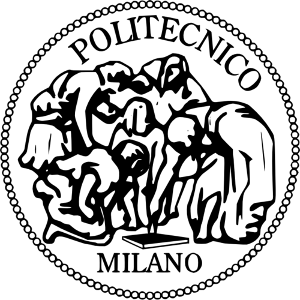
\includegraphics[width=0.3\textwidth]{./LogoPolimi.png}~\\[1cm]

\textsc{\LARGE Politecnico di Milano}\\[1cm]
\textsc{\LARGE Dipartimento di Elettronica, Informazione e Bioingegneria}\\[1.5 cm]




\textsc{\Large Switching and Routing}\\[1cm]

% Title
{ \huge \bfseries IP lookup - Bitmap algorithm \\[1.5cm] }

% Author and supervisor
\begin{texto}[6cm]
Grupo 4:\\
Nuno \textsc{Bajanca}\\
Vladimir  \textsc{Tomov}\\
Konstantin  \textsc{Tsolev}\\
Francisco  \textsc{Santos}\\
Alim  \textsc{Mohamed}\\
\end{texto}

\begin{texto}[6cm]
Professors:\\
Guido \textsc{Maier}\\
Navin   \textsc{Kukreja}\\
\end{texto}


\vfill

% Bottom of the page
{\large \today}

\end{center}
\end{titlepage}
\pagenumbering{roman}

\tableofcontents
\listoffigures
\listoftables

\chapter{Introduction}
This course project is a team assignment to design network of multiple switches, each with a different subnet mask, and implement Binary Trie and Bitmap IP lookup algorithms.

To take conclusions on the performance of these two algorithms the performance metrics are going to be discussed and the Lookup speed is going to be tested.

In this documentation file we will start by providing a basic theoretical introduction to the components, tools and algorithms that are being used or developed in this project. 

We will then explain the decisions relevant for the implementation of this project.

To end we will analyse the results obtained and conclude on them.

In the Annex section there is a Tutorial on how to run this project.

\pagenumbering{arabic}
\chapter{Theoretical Basis}
This chapter is dedicated to the introduction of the Theoretical principles behind the algorithms and to the introduction of the tools used in this project. 
\section{SDN}
SDN (Software Defined Networking) is a network architecture that breaks the vertical integration by separating the control logic (control plane) from the underlying routers and switches that will become simple forwarding elements (data plane). 
The main pillars of SDN are:
\begin{enumerate}
\item The control and data planes are decoupled;
\item Forwarding decisions are flow-based instead of destination-based;
\item Control logic is moved to an external entity, called SDN controller or NOS (Network Operating System);
\item Network is programmable through applications running on top of the controller (the fundamental characteristic of SDN).
\end{enumerate}

The SDN Architecure is represented in the figure \ref{fig:sdn}. In order to put all the theory into practice, we will use Mininet, that is explained in the following section.

\begin{minipage}{\linewidth}% to keep image and caption on one page

\makebox[\linewidth]{%to center the image
  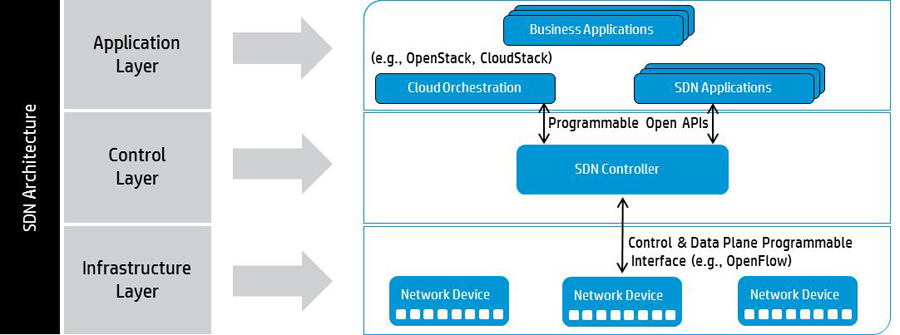
\includegraphics[width=\textwidth]{./sdn.png}
  }
\captionof{figure}{SDN Architecture [source: http://networkstatic.net/hp-announces-their-sdn-controller/]}\label{fig:sdn}
\end{minipage}


\section{Mininet}

Mininet is a virtual network environment that runs on a single machine and provides many of the OpenFlow features built-in. Mininet will emulate an entire network of switches, virtual hosts (running standard Linux software), the links between them and, optionally, a SDN controller.

Mininet supports research, development, learning, prototyping, testing, debugging, and any other tasks that could benefit from having a complete experimental network on a laptop or other PC.

\subsection{Why Mininet?} 
Among the multiple advantages that provides Mininet,some of the keys points that motivated its use for our project are:
\begin{itemize}
\item Mininet provides fast network setup, easy to use, custom topologies;
\item Mininet can run real Linux programs;
\item Mininet switches support OpenFlow;
\item Mininet is Open source, under active development.
\end{itemize}


\section{OpenFlow}

OpenFlow (OF) is considered one of the first software-defined networking (SDN) standards. It originally defined the communication protocol in SDN environments that enables the SDN Controller to directly interact with the forwarding plane of network devices such as switches and routers. The arquitecture of a switch network is demonstrated in figure \ref{fig:OF}. 

\begin{minipage}{\linewidth}% to keep image and caption on one page

\makebox[\linewidth]{%to center the image
  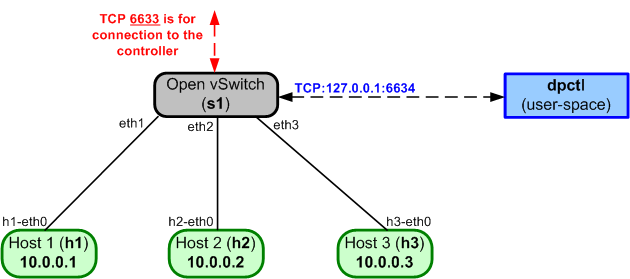
\includegraphics[width=\textwidth]{./of.png}
  }
\captionof{figure}{OpenFlow switch network arquitecture [source: http://www.costiser.ro]}\label{fig:OF}
\end{minipage}

Most OpenFlow switches have a passive listening port running on TCP 6633 (by default) that can be used to poll flows and counters or to manually insert flow entries.
 
The open flow hardware consists of the following:
\begin{itemize}
\item A flow table, represented in figure \ref{fig:OFtable}, containing flow entries consisting of match rules and actions that take on active flows;
\item A transport layer protocol that securely communicates with a controller about new entries that are not currently in the flow table.
\end{itemize}

\begin{minipage}{\linewidth}% to keep image and caption on one page

\makebox[\linewidth]{%to center the image
  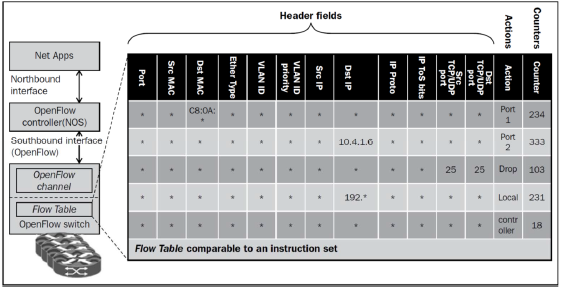
\includegraphics[width=\textwidth]{./of_table.png}
  }
\captionof{figure}{OpenFlow flow table}\label{fig:OFtable}
\end{minipage}

\section{Ryu Controller}

Ryu Controller, is an open software-defined networking (SDN) Controller designed to increase the agility of the network by making it easy to manage and adapt how traffic is handled. In general, the SDN Controller is the “brains” of the SDN environment, communicating information “down” to the switches and routers with southbound APIs, and “up” to the applications and business logic with northbound APIs. The Ryu Controller is supported by NTT and is deployed in NTT cloud data centers as well.

The Ryu Controller provides software components, with well-defined application program interfaces (APIs), that make it easy for developers to create new network management and control applications. This component approach helps organizations customize deployments to meet their specific needs; developers can quickly and easily modify existing components or implement their own to ensure the underlying network can meet the changing demands of their applications.



\subsection{How a Ryu Controller Fits in SDN environments}

Written entirely in Python, all of Ryu’s code is available under the Apache 2.0 license and open for anyone to use. The Ryu Controller supports NETCONF and OF-config network management protocols, as well as OpenFlow, which is one of the first and most widely deployed SDN communications standards.

The Ryu Controller can use OpenFlow to interact with the forwarding plane (switches and routers) to modify how the network will handle traffic flows, has showned in the figure \ref{fig:Ryu}. It has been tested and certified to work with a number of OpenFlow switches.

\begin{minipage}{\linewidth}% to keep image and caption on one page

\makebox[\linewidth]{%to center the image
  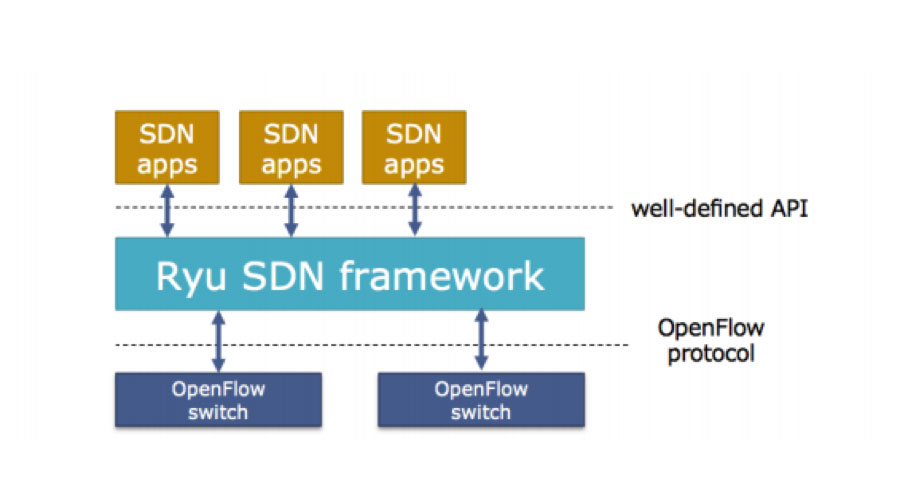
\includegraphics[width=\textwidth]{./ryu.jpg}
  }
\captionof{figure}{Ryu in SDN [source: https://www.sdxcentral.com]}\label{fig:Ryu}
\end{minipage}

\section{IP lookup}
\subsection{Performance metrics}
	During the analysis of the algorithms we will focus our attention to lookup speed, storage requirement and update time. It’s important to refer that Scalability and Flexibility are important performance metrics, but not relevant in this case to compare bitmap and binary trie algorithms.
\subsubsection{Lookup speed}
	The lookup speed is becoming more important every time advancements in the link bandwidth are made. The algorithms that are analysed in this project are slow when compared with hardware implementations, and for that reason they aren’t usually used in backbone routers.
\subsubsection{Storage requirement}
	In order to have fast memory access speed and low power consumption we need to assure small storage. For cache-based software algorithm this is very relevant.
\subsubsection{Update time (of lookup tables)}
	Nowadays the number of updates of lookup tables is increasing and they shouldn’t interfere with normal lookup operations.     
\subsubsection{Scalability}
	The size of the forwarding tables is increasing at a speed of approximately 25k entries per year so the algorithms should be able to support large forwarding tables. 
\subsubsection{Flexibility in implementation}
	Most of the algorithms can be implemented in different ways, and either software or hardware. These flexibility is important.


\subsection{Binary Trie algorithm}
	The Binary trie algorithm is based on binary tree structure. In this structure every node contains next hop information plus pointer to child nodes if there are any. If there is a default switch its information would be in the root node. 
	
Each node has two arcs:
\begin{itemize}
\item “1” corresponds to the right arc of the tree;
\item “0” corresponds to the left arc of the tree.
\end{itemize}
	
Each arc is terminated by node:
\begin{itemize}
\item If the node corresponds to a Prefix entry is marked as grey node;
\item If not it is marked as a white node.
\end{itemize}

White nodes must have at least one child rather grey node can be without any.

Route lookup is done by simply search for the longest prefix match by examining bit by bit of the ip address and matching it upon the tree. If longest prefix match is found algorithm returns the corresponding prefix, to that match. Otherwise binary trie algorithm performs backtrack to the last known prefix that was matched, which will be the longest match.

\subsubsection{Performance}
\begin{itemize}
\item Ip lookup speed, in the worst case, would be 32 memory accesses, O(W);
\item The worst update would translate in adding all the nodes so also 32, O(W);
\item Storing complexity would be, in the worst case, 32N*S, O(NW).
\end{itemize}

Where N is the number of prefixes, W the lenght of the prefixes (32 bits is maximum for ipv4) and S the memory space required for each node.

\subsection{Bitmap Tree algorithm}
The tree bitmap algorithm is based on multibit tree and it has bitmap compression to avoid wasting memory in the tree and achieve fast lookup.

In the bitmap tree each node has a fixed size containing a head pointer to the block of the child nodes, the extended bitmap for them, a head pointer to the next hop information and the extended bitmap for it. The update time is bounded by the size of the trie node and because of that the can’t be bigger than 8 otherwise the update would have a compromising cost. One of the key points of tree bitmap is the use of memory so each node is as small as possible in order to occupy the minimum memory possible. The child nodes of each node are stored contiguously in memory, there is only need to store one pointer and with help of the bitmap is possible to access to all of them. For the information of the next hop associated with the internal prefixes each node stores a head pointer and a bitmap for an array that stores that information and the array is associated to that node. The first bit of the bitmap is associated with the length 0, the second with the length 1 and so on.

To do the longest prefix match on the tree and according to the selected stride ( consider n) chosen we start to take the first n+1 bits of the prefix we want to search. Starting in the root node we search in the child bitmap, go to index correspondent to the bits we have and see if there is a ‘1’, that means that this node has a child. If there is a ‘1’ we need to see how many ‘1’ there are to the left to have the offset and then compute calculate the pointer to that child. Next, we check the internal bitmap to see the longest prefix. In first place we remove the rightmost bit and then go to the position that the bits we have corresponds and check to see if there is a ‘1 or not. If there is a ‘1’ it means that there is a prefix. We count the number of ‘1’ to the left to see the offset and then calculate the pointer and store it as prefix match. If there was a ‘0’ we just remove another bit and check it again, this is done until there are no more bits left. When the search in the internal bitmap is done we go the child node, and now we are taking the next n bits of the prefix we are searching and then do whole process again. We will keep doing this until there is no more children in the node we are or there are no more bits on the on prefix we have and then the search ends.

\subsubsection{Performance}
\begin{itemize}
\item Ip lookup speed, in the worst case, would be 32 memory accesses divided by the stride, O(W/k);
\item The update time is relatively fast but bounded by the size of the trie node, so no more than eight strides are used;
\item Storing complexity is good because both multi-bit tries and bitmap allow to reduce the wasted storage. 
\end{itemize}

Where W the lenght of the prefixes (32 bits is maximum for ipv4) and k the number of strides. This algorithm has a tradeoff between complexity and memory access, where the complexity is prefered is to the memory accesses.


\subsection{Comparison between algorithms}
Based on the theoretical introduction done in this section and general observations it is possible to conclude the following: 
\begin{itemize}
\item Bitmap algorithm uses fast search when compared to the binary trie;
\item Binary trie consumes more memory than bitmap.
\end{itemize}

Besides that bitmap has Scalability in terms of lookup speed and table size, the capability of high-speed updates, and feasibility in size to fit in a Level 3 forwarding engine or packet processor with low overhead.

During this project both algorithms will be implemented and the lookup speeds will be tested and compared.


\chapter{Implementation}
\section{Topology and configuration }
Our choice for topologies is listed in the table \ref{tab:topo}. 

\begin{minipage}{\linewidth}% to keep image and caption on one page
\captionof{table}{Topologies and distribution of ips}
\label{tab:topo}
\makebox[\linewidth]{%to center the image
  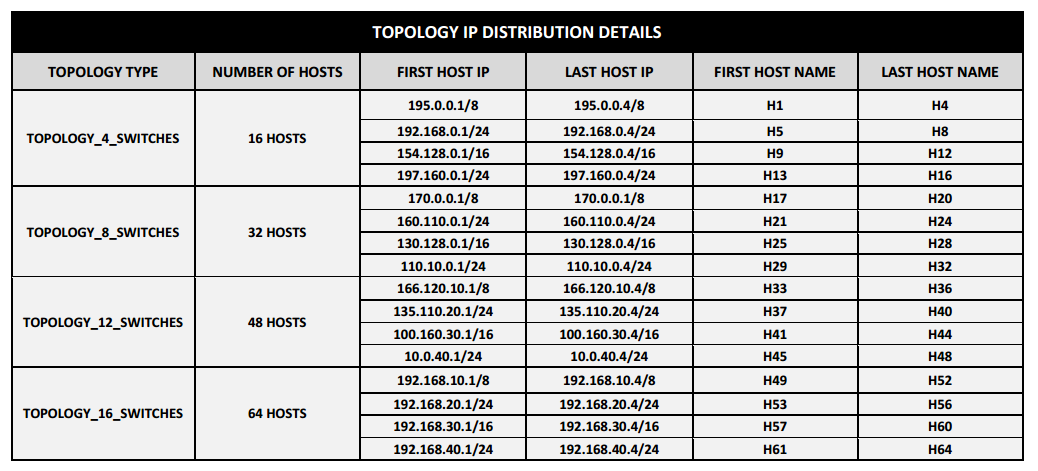
\includegraphics[width=\textwidth]{./topo.png}
  }
\end{minipage}

	There are allways 4 hosts per each switch, because the number of hosts in each switch is not relevant for the IP Lookup process.
	
The respectively distributed IPs are listed in the middle columns. In each topology 4 switches were introduced, two with a subnet of mask 255.255.255.0, one with a subnet mask of 255.255.0.0 and one with a subnet mask of 255.0.0.0. This allows the switches to be well distributed inside the trees.

Every host has a unique id and it is connected to the responding switch.
  
To apply these configurations to the project there are 4 different config and topology files. The information provided in them will be explained in the following lines.

\subsection{Configuration file}

The config file is usually associated with the topology file.It is the file which defines the ip adresses and default gateway distribution associated to a particular topology.

\subsection{Topology file}

The topology file defines the physical structure of the network.It defines the number of switches,hosts and interconnections between them.

\section{Controller}
The RYU controller was provided by the professor in the laboratory and the following changes were made:
\begin{itemize}
\item Constructor
\begin{itemize}
\item The switches and host static information was replaced by ReadingFromFile class that will the explained in section \ref{sec:config};
\item The two tries, that implement the algorithms, are created.
\end{itemize}
\item Packet Handler
\begin{itemize}
\item The lookup code was surronded by timers as explained in section \ref{sec:timers};
\item The lookup table search was replaced by two calls to the lookup algorithms implemented.
\end{itemize}
\end{itemize}


\section{Lookup algorithms}
In this section the implementation of the tree bitmap and binary trie algorithms are going to be explained. The UML for this implementation is the one in figure \ref{fig:UML}.

\subsection{Nodes}
The nodes are represented through classes.

In the Binary Trie all the nodes are equal, and represented by the class BinaryNode. This class has three references and a result. Being a binary trie we have the left and the right children, but as it is used for lookup.

In the Bitmap Tree the root node is different from the rest of the nodes, so there are used to classes for the nodes:
\begin{itemize}
\item Node - Has two bitmaps, the internal and the children’ one;
\item Root Node - Subclass of Node, besides being a node it also has two lists, the results and the children.
\end{itemize}
This is done because python doesn’t have pointers so we couldn’t alloc memory for the children of a node and get the first memory position, instead we use a list (works like a vector) and the first memory position, present in every node, is just the index of the first object.

\begin{minipage}{\linewidth}% to keep image and caption on one page

\makebox[\linewidth]{%to center the image
  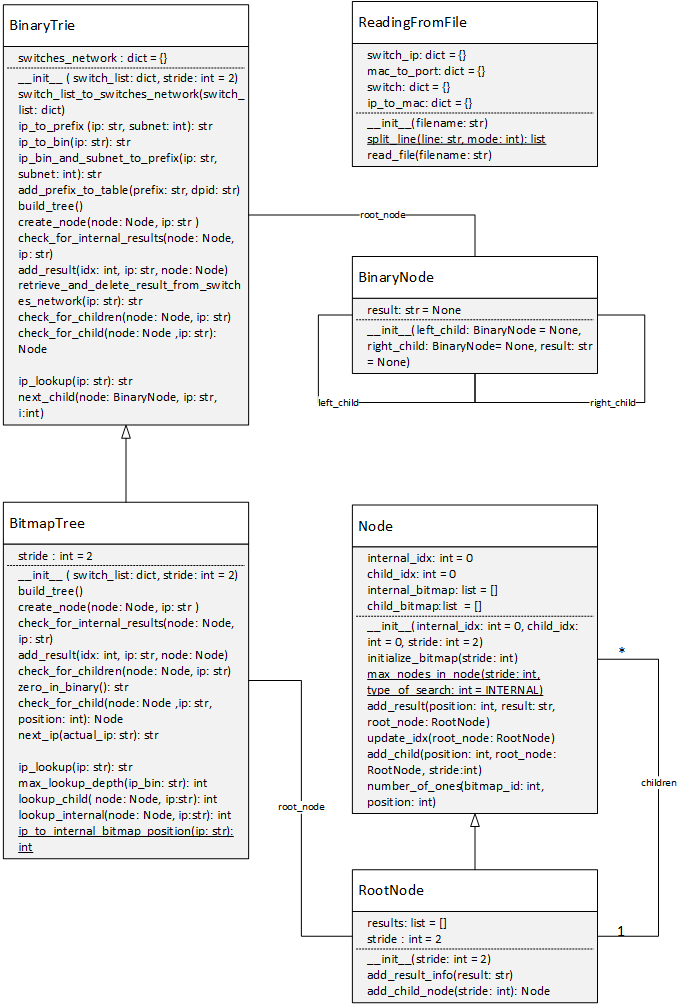
\includegraphics[width=\textwidth]{./uml.png}
  }
\captionof{figure}{UML}\label{fig:UML}
\end{minipage}

\subsection{Tree Creation}
Both algorithms have the same fluxogram, represented in figure \ref{fig:flux}, for the construction of the tree so the Bitmap Tree is a subclass of the Binary Trie. This assures that all the methods done in the Binary  Trie are either used or overridden by the Bitmap Tree.

\begin{minipage}{\linewidth}% to keep image and caption on one page

\makebox[\linewidth]{%to center the image
  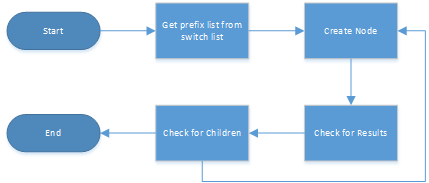
\includegraphics[width=0.8\textwidth]{./flux.png}
  }
\captionof{figure}{Fluxogram for the Tree Creation}\label{fig:flux}
\end{minipage}

The construction of the trees starts with the conversion of the switch list to a prefix table in the method switch\textunderscore list\textunderscore to\textunderscore switches\textunderscore network(). This method converts the switch ips to binary and then trims them using the prefix information (mask).

Next, the root\textunderscore node is created. For both algorithms this is a simple call to the constructor of the respective class.
From now on the construction of the trees differs so we will explain them in separate sub-chapters.

\subsubsection{Binary Trie}
The creation of the nodes in the binary trie is done in a recursive way starting by the left nodes, this means that the first node to be constructed is “0” (if there is any prefix that starts with it, obviously) and then “00” and so on until there is no prefix correspondence. When that happens the algorithm starts returning and constructing the right nodes until all the prefixes are represented in the nodes.
	
The sequence of methods called in the code are the following: 
\begin{enumerate}
\item create\textunderscore node() : A method that will them call:
\begin{enumerate}
\item check\textunderscore for\textunderscore results() : If an exact match between the ip of the node and one switch in the list is found then that result is added to the node;
\item check\textunderscore for\textunderscore children(): Checks for a child in the left node, if it finds one it will call create\textunderscore node() for it. If it doesn’t or if the create\textunderscore node() already returned then it will check for the right child, applying the same principle. 
\end{enumerate}
\end{enumerate}

In the print screen presented in the figure \ref{fig:print_controller} we can see that from the node “0110” we build all the nodes to the left (“01100” and its children) and only after we return to the “0110” and we start to build to the right (“01101” and its children).

\begin{minipage}{\linewidth}% to keep image and caption on one page

\makebox[\linewidth]{%to center the image
  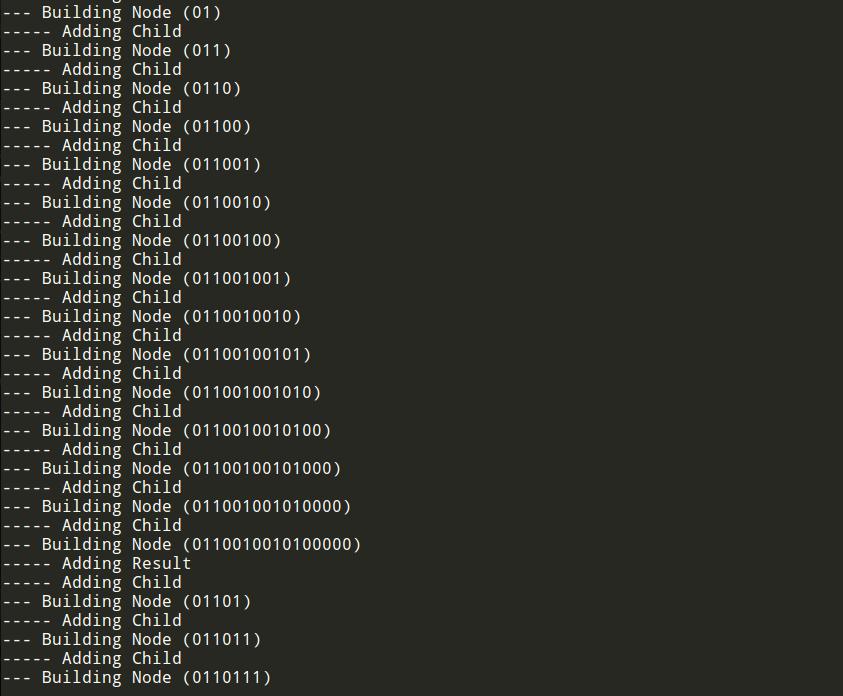
\includegraphics[width=\textwidth]{./print_controller.png}
  }
\captionof{figure}{Print screen from controller building the binary trie for the configuration with 16 switches}\label{fig:print_controller}
\end{minipage}

\subsubsection{Bitmap Tree}
The same logic of the Binary Trie is applied but in this case the implementation is more complex and requires the help of the following methods:
\begin{itemize}
\item zero\textunderscore in\textunderscore binary() : This method returns the zero in binary according to the stride so, for example, if stride is 2 this method returns “000”, that corresponds to the first child associated with this node;
\item next\textunderscore ip() :This method returns the next\textunderscore ip and works for both type of searches:
\begin{itemize}
\item For internal result search the “binary tree”(There isn’t any binary tree, but the works as there is) in snake like movement (“”->“0”->”1”->”00”->”11”->..);
\item For child search the “binary tree” is searched only on one level (for ex: from “000” to “111”)
\end{itemize}
\end{itemize}

In the create\textunderscore node() method we start by searching for results in the check\textunderscore for\textunderscore internal\textunderscore results() method, which used next\textunderscore ip() to go true all the possible correspondences in the prefix table. If an “exact match” is found a “1” is putted in the correspondent position in the internal bitmap and the correspondent is deleted from the prefix table and added to the result list (the results are appended in sequence so the index in the node corresponds to the first result in the node in question).

After the internal search we start searching for children. When a child is found it is added to the list and a “1” is putted in the bitmap. To assure the index stays correct we search all children from a certain node and only after finishing the search we do a second loop (only through the children found) where we enter the recursive, calling the create\textunderscore node() method for that child.

In the print screen presented in the figure \ref{fig:print_controller2} we can see that for the Root Node we found several results (as the stride is 8 we can conclude that the switches 9, 5, 13 and 1 have a 255.0.0.0 mask) and only after that we search for children. After finding all the children we went to the first child and repeated the process, not finding any result but finding at least one result.



\begin{minipage}{\linewidth}% to keep image and caption on one page

\makebox[\linewidth]{%to center the image
  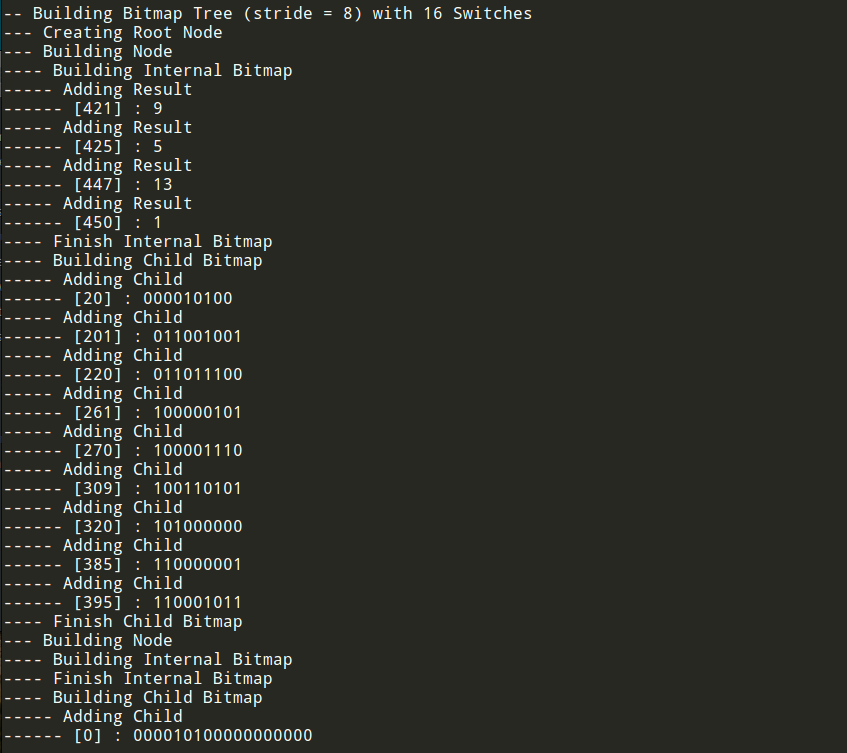
\includegraphics[width=\textwidth]{./print_controller2.png}
  }
\captionof{figure}{Print screen from controller building the Bitmap Tree for the configuration with 16 switches}\label{fig:print_controller2}
\end{minipage}

It’s important to refer that the prefix table gets its entries deleted when they are added to the tree. This is a responsibility of the method retrieve\textunderscore and\textunderscore delete\textunderscore result\textunderscore from\textunderscore switches\textunderscore network() which is shared by class and subclass.

\subsection{Lookup implementation}

The lookup in both algorithms is implemented precisely as described in the theoretical section of this documentation.

\subsubsection{Binary Trie}

For the binary trie the ip\textunderscore lookup we need backtrack so a recursive function was implemented for the search:
\begin{enumerate}
\item Starting from the root node the trie is crossed until the last node in the path of the ip received is reached;
\item The recursive method returns:
\begin{enumerate}
\item The next-hop information present in its structure (None if it’s a gray node);
\item The next-hop information returned by the child node, if it is not None.
\end{enumerate}
\end{enumerate}

In this way when the end of the recursive is reached we will have the longest match switch information.


\subsubsection{Bitmap Tree}
In the bitmap case no backtracking is needed so we a loop. The loop is between the following methods:
\begin{enumerate}
\item lookup\textunderscore child(): In this method we look for the next node, if it exists, the position(index in the bitmap plus the number of ones) is saved;
\item lookup\textunderscore internal(): In this method we look for the longest match prefix in the bitmap, this makes this method to be also a loop. When, and if, a match is found the position is saved.
\end{enumerate}
If a child is found the same procedure is done in it, if it isn’t than the last result obtained is returned.


\section{Reading Configuration File}
\label{sec:config}
	Instead of having to do manually the creation of the topology of the network we read the config file and generate the topology. In the reading of the file we take all the information about the switches we need (IP, Mask, id) and then associate a sequential MAC address to each one and create the switch\textunderscore ip list and the switch list. We also read the ip of the hosts and to which switch they are connected. We also assign sequentially a MAC address to each one and then create the ip\textunderscore to\textunderscore mac list and mac\textunderscore to\textunderscore port list.
	
	In order to do this we basically use to methods:
\begin{itemize}
\item split\textunderscore line(): This method receives the lines from the config file and returns a list with the important values that we need;
\item read\textunderscore file(): This method first stores the information in the config file to a general buffer and then puts it in the specific dictionaries that we want assigning sequentially the MAC addresses needed;
\end{itemize}


\section{Timers}
\label{sec:timers}
\subsection{Timers in the controler  }

Timers were implemented in the code to obtain the following results:
\begin{itemize}
\item The lookup time;
\item The percentage of time needed to respond to an incoming packet that is spent in the lookup algorithm.
\end{itemize}
Having this is consideration there are two timers:
\begin{enumerate}
\item Starting when a packet is received, finished when the packet is forward. This timer is ignored if the packet doesn’t require ip lookup, for example arp requests;
\item Starting when the ip lookup starts and finishing when the next-op information is obtained.
\end{enumerate}
 
For the correct analysis of the performance both algorithms are performed in the same response. We will then obtain the following values, for each request:

\begin{itemize}
\item processing
\item lookup\textunderscore bitmap
\item lookup\textunderscore trie
\end{itemize}




And we compute the following values:
\begin{itemize}
\item processing\textunderscore bitmap = processing - lookup\textunderscore trie
\item processing\textunderscore trie = processing  - lookup\textunderscore bitmap
\item lookup\textunderscore percentage\textunderscore bitmap = (lookup\textunderscore bitmap/processing\textunderscore bitmap)
\item lookup\textunderscore percentage\textunderscore trie = (lookup\textunderscore trie/processing\textunderscore trie)
\end{itemize} 



\subsection{Timers average via Rest API}
To make the Lookup time performance metric easier to evaluate the results are presented through the RYU Rest API. For these the method list\textunderscore timers() was added to the class LookupController with the route '/v1.0/lookup/timers'.

In this class, beside having the value of the timers, it was also added some code to make averages and changing the units, so a response to a GET request is:

\begin{itemize}
\item average\textunderscore lookup\textunderscore bitmap (ms)
\item average\textunderscore lookup\textunderscore trie (ms)
\item average\textunderscore processing\textunderscore bitmap (ms)
\item average\textunderscore processing\textunderscore trie (ms)
\item average\textunderscore lookup\textunderscore percentage\textunderscore bitmap (\%)
\item average\textunderscore lookup\textunderscore percentage\textunderscore trie (\%)
\item lookup\textunderscore bitmap (table - values in s)
\item lookup\textunderscore trie (table - values in s)
\end{itemize}




\chapter{Results}
We derived several conclusions from the timers implemented, starting from the stride until the comparison between the two algorithms. This results were split in different sections, presented in this chapter.


\section{Stride}
From the results in the table \ref{tab:stride_table} we can understand that the lookup decreases with the stride. This proves the lookup performance assumption that it is O(W/k) being k the stride and W the number of bits.

We chose to use stride of 8 for the rest of the tests but it is relevant to understand that we are not accessing the update time, which becomes worse with bigger strides.



\begin{minipage}{\linewidth}% to keep image and caption on one page
\captionof{table}{Lookup time for different stride values in the 4 switches configuration.}
\label{tab:stride_table}
\makebox[\linewidth]{%to center the image
  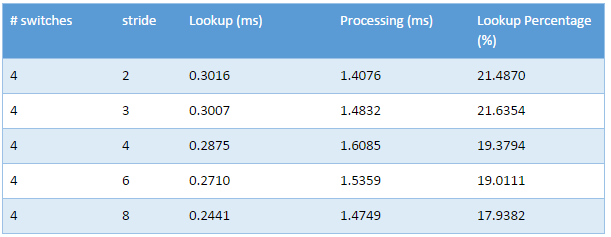
\includegraphics[width=\textwidth]{./stride_table.png}
  }
\end{minipage}

\section{Network sizes}
	The table \ref{tab:size_table} shows the difference between in the lookup time in different topologies. This results goes against what was supposed because there is a clear deterioration of the lookup time with the number of switches. 
As explained before the number of switches should only influence the Storage but in according to the results they influence the results. One explanation for this is related to the fact that the bitmap representation used is a list and so the time spent in counting the number of ones every time a result or a child is found its significant.





\begin{minipage}{\linewidth}% to keep image and caption on one page
\captionof{table}{Lookup time for different switches configuration.}
\label{tab:size_table}
\makebox[\linewidth]{%to center the image
  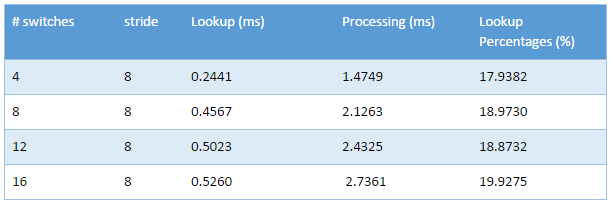
\includegraphics[width=\textwidth]{./size_table.png}
  }
\end{minipage}

\section{Binary vs Bitmap}
	Once again there are discrepancies in the results because the bitmap algorithm should be faster than the binary one. 
	
For these results, presented in table \ref{tab:algorithms_table}, the explanation is related to the way the speed of the algorithm was evaluated. The speed is evaluated through memory accesses, and in fact bitmap has less accesses to memory, but it doesn’t take into account the tradeoff introduced by bitmap that is the complexity.

 

\begin{minipage}{\linewidth}% to keep image and caption on one page
\captionof{table}{Lookup time for Bitmap and Binary}
\label{tab:algorithms_table}
\makebox[\linewidth]{%to center the image
  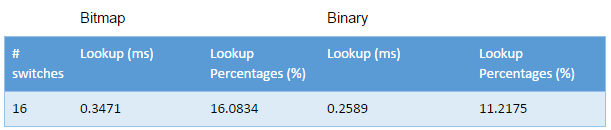
\includegraphics[width=\textwidth]{./algorithms_table.png}
  }
\end{minipage}


\chapter{Conclusions}
In a conclusion manner, we were able to complete the objectives proposed:
\begin{itemize}
\item Design of 4 network topologies, each one with a different number of switches and a different subnet mask;
\item Implement the two lookup algorithms, Binary Trie and Bitmap Tree;
\item Measure performance parameters on these algorithms.
\end{itemize}
Unfortunately the tools used, and the implementation done didn’t allowed the results to reach the theoretical conclusions, but these discrepancies were explained in the result analyze section. 

We can then conclude that for mininet running on a linux virtual machine the complex lookup computations of bitmap don’t compensate the reduction in memory accesses.

We consider that this project was very important for the better understanding of SDN and to learn how to work with new tools, as mininet and RYU, that we will possible use in the future.


\chapter{Bibliography}
\begin{enumerate}
	\item H.J. Chao, B. Liu, High Performance Switches and Routers, John Wiley \& Sons, 2007;
	\item Theoretical classes slides;
	\item Mininet - http://mininet.org/;
	\item OpenFlow - https://www.opennetworking.org/sdn-resources/openflow;
	\item RYU SDN Framework - http://osrg.github.io/ryu/.
\end{enumerate}



\end{document}